% Options for packages loaded elsewhere
\PassOptionsToPackage{unicode}{hyperref}
\PassOptionsToPackage{hyphens}{url}
%
\documentclass[
]{book}
\usepackage{amsmath,amssymb}
\usepackage{lmodern}
\usepackage{ifxetex,ifluatex}
\ifnum 0\ifxetex 1\fi\ifluatex 1\fi=0 % if pdftex
  \usepackage[T1]{fontenc}
  \usepackage[utf8]{inputenc}
  \usepackage{textcomp} % provide euro and other symbols
\else % if luatex or xetex
  \usepackage{unicode-math}
  \defaultfontfeatures{Scale=MatchLowercase}
  \defaultfontfeatures[\rmfamily]{Ligatures=TeX,Scale=1}
\fi
% Use upquote if available, for straight quotes in verbatim environments
\IfFileExists{upquote.sty}{\usepackage{upquote}}{}
\IfFileExists{microtype.sty}{% use microtype if available
  \usepackage[]{microtype}
  \UseMicrotypeSet[protrusion]{basicmath} % disable protrusion for tt fonts
}{}
\makeatletter
\@ifundefined{KOMAClassName}{% if non-KOMA class
  \IfFileExists{parskip.sty}{%
    \usepackage{parskip}
  }{% else
    \setlength{\parindent}{0pt}
    \setlength{\parskip}{6pt plus 2pt minus 1pt}}
}{% if KOMA class
  \KOMAoptions{parskip=half}}
\makeatother
\usepackage{xcolor}
\IfFileExists{xurl.sty}{\usepackage{xurl}}{} % add URL line breaks if available
\IfFileExists{bookmark.sty}{\usepackage{bookmark}}{\usepackage{hyperref}}
\hypersetup{
  pdftitle={LIN 380 Coursebook},
  pdfauthor={Jerid Francom},
  hidelinks,
  pdfcreator={LaTeX via pandoc}}
\urlstyle{same} % disable monospaced font for URLs
\usepackage{color}
\usepackage{fancyvrb}
\newcommand{\VerbBar}{|}
\newcommand{\VERB}{\Verb[commandchars=\\\{\}]}
\DefineVerbatimEnvironment{Highlighting}{Verbatim}{commandchars=\\\{\}}
% Add ',fontsize=\small' for more characters per line
\usepackage{framed}
\definecolor{shadecolor}{RGB}{248,248,248}
\newenvironment{Shaded}{\begin{snugshade}}{\end{snugshade}}
\newcommand{\AlertTok}[1]{\textcolor[rgb]{0.94,0.16,0.16}{#1}}
\newcommand{\AnnotationTok}[1]{\textcolor[rgb]{0.56,0.35,0.01}{\textbf{\textit{#1}}}}
\newcommand{\AttributeTok}[1]{\textcolor[rgb]{0.77,0.63,0.00}{#1}}
\newcommand{\BaseNTok}[1]{\textcolor[rgb]{0.00,0.00,0.81}{#1}}
\newcommand{\BuiltInTok}[1]{#1}
\newcommand{\CharTok}[1]{\textcolor[rgb]{0.31,0.60,0.02}{#1}}
\newcommand{\CommentTok}[1]{\textcolor[rgb]{0.56,0.35,0.01}{\textit{#1}}}
\newcommand{\CommentVarTok}[1]{\textcolor[rgb]{0.56,0.35,0.01}{\textbf{\textit{#1}}}}
\newcommand{\ConstantTok}[1]{\textcolor[rgb]{0.00,0.00,0.00}{#1}}
\newcommand{\ControlFlowTok}[1]{\textcolor[rgb]{0.13,0.29,0.53}{\textbf{#1}}}
\newcommand{\DataTypeTok}[1]{\textcolor[rgb]{0.13,0.29,0.53}{#1}}
\newcommand{\DecValTok}[1]{\textcolor[rgb]{0.00,0.00,0.81}{#1}}
\newcommand{\DocumentationTok}[1]{\textcolor[rgb]{0.56,0.35,0.01}{\textbf{\textit{#1}}}}
\newcommand{\ErrorTok}[1]{\textcolor[rgb]{0.64,0.00,0.00}{\textbf{#1}}}
\newcommand{\ExtensionTok}[1]{#1}
\newcommand{\FloatTok}[1]{\textcolor[rgb]{0.00,0.00,0.81}{#1}}
\newcommand{\FunctionTok}[1]{\textcolor[rgb]{0.00,0.00,0.00}{#1}}
\newcommand{\ImportTok}[1]{#1}
\newcommand{\InformationTok}[1]{\textcolor[rgb]{0.56,0.35,0.01}{\textbf{\textit{#1}}}}
\newcommand{\KeywordTok}[1]{\textcolor[rgb]{0.13,0.29,0.53}{\textbf{#1}}}
\newcommand{\NormalTok}[1]{#1}
\newcommand{\OperatorTok}[1]{\textcolor[rgb]{0.81,0.36,0.00}{\textbf{#1}}}
\newcommand{\OtherTok}[1]{\textcolor[rgb]{0.56,0.35,0.01}{#1}}
\newcommand{\PreprocessorTok}[1]{\textcolor[rgb]{0.56,0.35,0.01}{\textit{#1}}}
\newcommand{\RegionMarkerTok}[1]{#1}
\newcommand{\SpecialCharTok}[1]{\textcolor[rgb]{0.00,0.00,0.00}{#1}}
\newcommand{\SpecialStringTok}[1]{\textcolor[rgb]{0.31,0.60,0.02}{#1}}
\newcommand{\StringTok}[1]{\textcolor[rgb]{0.31,0.60,0.02}{#1}}
\newcommand{\VariableTok}[1]{\textcolor[rgb]{0.00,0.00,0.00}{#1}}
\newcommand{\VerbatimStringTok}[1]{\textcolor[rgb]{0.31,0.60,0.02}{#1}}
\newcommand{\WarningTok}[1]{\textcolor[rgb]{0.56,0.35,0.01}{\textbf{\textit{#1}}}}
\usepackage{longtable,booktabs,array}
\usepackage{calc} % for calculating minipage widths
% Correct order of tables after \paragraph or \subparagraph
\usepackage{etoolbox}
\makeatletter
\patchcmd\longtable{\par}{\if@noskipsec\mbox{}\fi\par}{}{}
\makeatother
% Allow footnotes in longtable head/foot
\IfFileExists{footnotehyper.sty}{\usepackage{footnotehyper}}{\usepackage{footnote}}
\makesavenoteenv{longtable}
\usepackage{graphicx}
\makeatletter
\def\maxwidth{\ifdim\Gin@nat@width>\linewidth\linewidth\else\Gin@nat@width\fi}
\def\maxheight{\ifdim\Gin@nat@height>\textheight\textheight\else\Gin@nat@height\fi}
\makeatother
% Scale images if necessary, so that they will not overflow the page
% margins by default, and it is still possible to overwrite the defaults
% using explicit options in \includegraphics[width, height, ...]{}
\setkeys{Gin}{width=\maxwidth,height=\maxheight,keepaspectratio}
% Set default figure placement to htbp
\makeatletter
\def\fps@figure{htbp}
\makeatother
\setlength{\emergencystretch}{3em} % prevent overfull lines
\providecommand{\tightlist}{%
  \setlength{\itemsep}{0pt}\setlength{\parskip}{0pt}}
\setcounter{secnumdepth}{5}
% default
\usepackage{booktabs}
\usepackage{amsthm}
\usepackage{float}
\makeatletter
\def\thm@space@setup{%
  \thm@preskip=8pt plus 2pt minus 4pt
  \thm@postskip=\thm@preskip
}
\makeatother

% added
\usepackage{longtable}
\usepackage{framed,color}
\definecolor{shadecolor}{RGB}{248,248,248}

\ifxetex
  \usepackage{letltxmacro}
  \setlength{\XeTeXLinkMargin}{2pt}
  \LetLtxMacro\SavedIncludeGraphics\includegraphics
  \def\includegraphics#1#{% #1 catches optional stuff (star/opt. arg.)
    \IncludeGraphicsAux{#1}%
  }%
  \newcommand*{\IncludeGraphicsAux}[2]{%
    \XeTeXLinkBox{%
      \SavedIncludeGraphics#1{#2}%
    }%
  }%
\fi

\newenvironment{rmdblock}[1]
  {\begin{shaded*}
  \begin{itemize}
  \renewcommand{\labelitemi}{
    \raisebox{-.5\height}[0pt][0pt]{
      {\setkeys{Gin}{width=2em,keepaspectratio}\includegraphics{assets/images/#1}}
    }
  }
  \item
  }
  {
  \end{itemize}
  \end{shaded*}
  }
\newenvironment{rmdkey}
  {\begin{rmdblock}{key}}
  {\end{rmdblock}}
\newenvironment{rmdnote}
  {\begin{rmdblock}{note}}
  {\end{rmdblock}}
\newenvironment{rmdtip}
  {\begin{rmdblock}{tip}}
  {\end{rmdblock}}
\newenvironment{rmdwarning}
  {\begin{rmdblock}{warning}}
  {\end{rmdblock}}
\newenvironment{rmdactivity}
  {\begin{rmdblock}{code}}
  {\end{rmdblock}}

\ifluatex
  \usepackage{selnolig}  % disable illegal ligatures
\fi
\usepackage[]{natbib}
\bibliographystyle{apalike}

\title{LIN 380 Coursebook}
\author{Jerid Francom}
\date{2021-04-20}

\begin{document}
\maketitle

{
\setcounter{tocdepth}{1}
\tableofcontents
}
\hypertarget{about}{%
\chapter*{About}\label{about}}
\addcontentsline{toc}{chapter}{About}

\ldots{}

\hypertarget{part-welcome}{%
\part{Welcome}\label{part-welcome}}

\hypertarget{course-overview}{%
\chapter*{Overview}\label{course-overview}}
\addcontentsline{toc}{chapter}{Overview}

\hypertarget{about-this-course}{%
\chapter*{About this course}\label{about-this-course}}
\addcontentsline{toc}{chapter}{About this course}

\hypertarget{description}{%
\section*{Description}\label{description}}
\addcontentsline{toc}{section}{Description}

\hypertarget{conventions}{%
\section*{Conventions}\label{conventions}}
\addcontentsline{toc}{section}{Conventions}

This book is about the concepts for understanding and the techniques for doing quantitative language science. Therefore there will be an intermingling of prose and code presented. As such, an attempt to establish consistent conventions throughout the text has been made to signal reader's attention as appropriate. As we explore concepts, R code itself will be incorporated into the text. This may be a unique textbook compared to others you have seen. It has been created using R itself --specifically using an R language package called \texttt{bookdown} \citep{R-bookdown}. This R package makes it possible to write, execute (`run'), and display code and results within the text.

For example, the following text block shows actual R code and the results that are generated when running this code. Note that the hashtag \texttt{\#} signals a \textbf{code comment}. The code follows within the same text block and a subsequent text block displays the output of the code.

\begin{Shaded}
\begin{Highlighting}[]
\CommentTok{\# Add 1 plus 1}
\DecValTok{1} \SpecialCharTok{+} \DecValTok{1}
\end{Highlighting}
\end{Shaded}

\begin{verbatim}
## [1] 2
\end{verbatim}

Inline code will be used when code blocks are short and the results are not needed for display. For example, the same code as above will sometimes appear as \texttt{1\ +\ 1}.

When necessary meta-description of code will appear. This is particularly relevant for R Markdown documents.

\begin{verbatim}
```{r test-code}
1 + 1
```
\end{verbatim}

In terms of prose, key concepts will be signaled using \textbf{\emph{bold italics}}. Terms that appear in this typeface will also appear in the {[}glossary{]} at the end of the text. Furthermore, there are four pose text blocks that will be used to signal the reader's attention: \emph{key points}, \emph{notes}, \emph{tips}, and \emph{warnings}.

Key points summarize the main points to be covered in a chapter or a subsection of the text.

\begin{rmdkey}
In this chapter you will learn:

\begin{itemize}
\tightlist
\item
  the goals of this textbook
\item
  the reasoning for using the R programming language
\item
  important text conventions employed in this textbook
\end{itemize}
\end{rmdkey}

Notes provide a bit more information on the topic or where to find more information.

\begin{rmdnote}
R is more than a powerful statistical programming language, it also can
be used to perform all the necessary steps in a data science project;
including reporting. A relatively new addition to the reporting
capabilities of R is the \texttt{bookdown} package (this textbook was
created using this very package). You can find out more
\href{https://bookdown.org/}{here}.
\end{rmdnote}

Tips are used to signal helpful hints that might otherwise be overlooked.

\begin{rmdtip}
During a the course of an exploratory work session, many R objects are
often created to test ideas. At some point inspecting the workspace
becomes difficult due to the number of objects displayed using
\texttt{ls()}.

To remove all objects from the workspace, use
\texttt{rm(list\ =\ ls())}.
\end{rmdtip}

Errors will be an inevitable part of learning, but some errors can be avoided. The text will used the warning text block to highlight typical pitfalls and errors.

\begin{rmdwarning}
Hello world!\\
This is a warning.
\end{rmdwarning}

Although this is not intended to be a in-depth introduction to statistical techniques, mathematical formulas will be included in the text. These formulas will appear either inline \(1 + 1 = 2\) or as block equations.

\begin{equation}
  \hat{c} = \underset{c \in C} {\mathrm{argmax}} ~\hat{P}(c) \prod_i \hat{P}(w_i|c)
  \label{eq:example-formula}
\end{equation}

Data analysis leans heavily on graphical representations. Figures will appear numbered, as in Figure \ref{fig:test-fig}.

\begin{Shaded}
\begin{Highlighting}[]
\FunctionTok{library}\NormalTok{(ggplot2) }\CommentTok{\# load graphics package}
\FunctionTok{ggplot}\NormalTok{(mtcars, }\FunctionTok{aes}\NormalTok{(}\AttributeTok{x =}\NormalTok{ hp, }\AttributeTok{y =}\NormalTok{ mpg)) }\SpecialCharTok{+} \CommentTok{\# map \textquotesingle{}hp\textquotesingle{} and \textquotesingle{}mpg\textquotesingle{} to coordinate space}
  \FunctionTok{geom\_point}\NormalTok{() }\SpecialCharTok{+} \CommentTok{\# add points}
  \FunctionTok{geom\_smooth}\NormalTok{(}\AttributeTok{method =} \StringTok{"lm"}\NormalTok{) }\SpecialCharTok{+} \CommentTok{\# draw linear trend line}
  \FunctionTok{labs}\NormalTok{(}\AttributeTok{x =} \StringTok{"Horsepower"}\NormalTok{, }\CommentTok{\# label x axis}
       \AttributeTok{y =} \StringTok{"Miles per gallon"}\NormalTok{, }\CommentTok{\# label y axis}
       \AttributeTok{title =} \StringTok{"Test plot"}\NormalTok{, }\CommentTok{\# add title}
       \AttributeTok{subtitle =} \StringTok{"From mtcars dataset"}\NormalTok{) }\CommentTok{\# add subtitle}
\end{Highlighting}
\end{Shaded}

\begin{verbatim}
## `geom_smooth()` using formula 'y ~ x'
\end{verbatim}

\begin{figure}
\centering
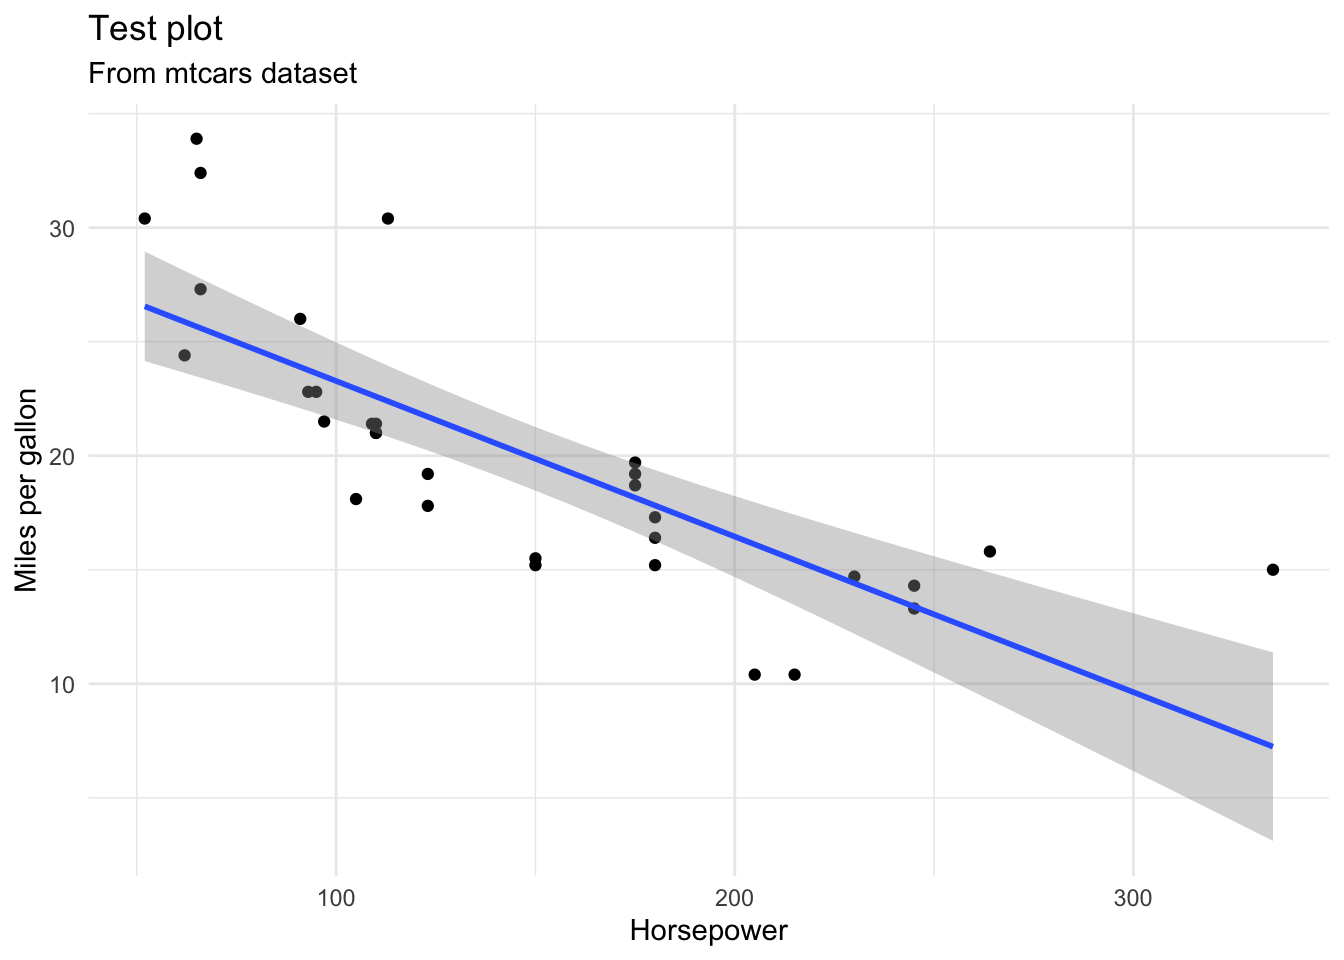
\includegraphics{01-course_files/figure-latex/test-fig-1.pdf}
\caption{\label{fig:test-fig}Test plot from mtcars dataset}
\end{figure}

Tables, such as Table \ref{tab:test-tab} will be numbered separately from figures.

\begin{Shaded}
\begin{Highlighting}[]
\NormalTok{knitr}\SpecialCharTok{::}\FunctionTok{kable}\NormalTok{(}
  \FunctionTok{head}\NormalTok{(iris, }\DecValTok{20}\NormalTok{), }\AttributeTok{caption =} \StringTok{\textquotesingle{}Here is a nice table!\textquotesingle{}}\NormalTok{,}
  \AttributeTok{booktabs =} \ConstantTok{TRUE}
\NormalTok{)}
\end{Highlighting}
\end{Shaded}

\begin{table}

\caption{\label{tab:test-tab}Here is a nice table!}
\centering
\begin{tabular}[t]{rrrrl}
\toprule{}
Sepal.Length & Sepal.Width & Petal.Length & Petal.Width & Species\\
\midrule{}
5.1 & 3.5 & 1.4 & 0.2 & setosa\\
4.9 & 3.0 & 1.4 & 0.2 & setosa\\
4.7 & 3.2 & 1.3 & 0.2 & setosa\\
4.6 & 3.1 & 1.5 & 0.2 & setosa\\
5.0 & 3.6 & 1.4 & 0.2 & setosa\\
\addlinespace
5.4 & 3.9 & 1.7 & 0.4 & setosa\\
4.6 & 3.4 & 1.4 & 0.3 & setosa\\
5.0 & 3.4 & 1.5 & 0.2 & setosa\\
4.4 & 2.9 & 1.4 & 0.2 & setosa\\
4.9 & 3.1 & 1.5 & 0.1 & setosa\\
\addlinespace
5.4 & 3.7 & 1.5 & 0.2 & setosa\\
4.8 & 3.4 & 1.6 & 0.2 & setosa\\
4.8 & 3.0 & 1.4 & 0.1 & setosa\\
4.3 & 3.0 & 1.1 & 0.1 & setosa\\
5.8 & 4.0 & 1.2 & 0.2 & setosa\\
\addlinespace
5.7 & 4.4 & 1.5 & 0.4 & setosa\\
5.4 & 3.9 & 1.3 & 0.4 & setosa\\
5.1 & 3.5 & 1.4 & 0.3 & setosa\\
5.7 & 3.8 & 1.7 & 0.3 & setosa\\
5.1 & 3.8 & 1.5 & 0.3 & setosa\\
\bottomrule{}
\end{tabular}
\end{table}

\hypertarget{r-and-rstudio}{%
\chapter*{R and RStudio}\label{r-and-rstudio}}
\addcontentsline{toc}{chapter}{R and RStudio}

\hypertarget{part-foundations}{%
\part{Foundations}\label{part-foundations}}

\hypertarget{foundations-overview}{%
\chapter*{Overview}\label{foundations-overview}}
\addcontentsline{toc}{chapter}{Overview}

\hypertarget{foundations}{%
\section*{Foundations}\label{foundations}}
\addcontentsline{toc}{section}{Foundations}

In this section, \ldots.

\hypertarget{introduction-to-text-analysis}{%
\chapter{Introduction to text analysis}\label{introduction-to-text-analysis}}

\begin{rmdkey}
In this chapter you will learn:

\begin{itemize}
\tightlist
\item
  the goals of this textbook
\item
  the reasoning for using the R programming language
\item
  important text conventions employed in this textbook
\end{itemize}
\end{rmdkey}

\hypertarget{quantitative-studies}{%
\section{Quantitative studies}\label{quantitative-studies}}

\hypertarget{quantitative-language-research}{%
\section{Quantitative language research}\label{quantitative-language-research}}

\hypertarget{text-analysis}{%
\subsection{Text analysis}\label{text-analysis}}

\hypertarget{section}{%
\subsection{\ldots{}}\label{section}}

\hypertarget{activities}{%
\chapter*{Activities}\label{activities}}
\addcontentsline{toc}{chapter}{Activities}

\hypertarget{part-orientation}{%
\part{Orientation}\label{part-orientation}}

\hypertarget{orientation-overview}{%
\chapter*{Overview}\label{orientation-overview}}
\addcontentsline{toc}{chapter}{Overview}

\hypertarget{understanding-data}{%
\chapter{Understanding data}\label{understanding-data}}

\begin{rmdkey}
In this chapter you will learn:

\begin{itemize}
\tightlist
\item
  the goals of this textbook
\item
  the reasoning for using the R programming language
\item
  important text conventions employed in this textbook
\end{itemize}
\end{rmdkey}

\hypertarget{section-1}{%
\section{\ldots{}}\label{section-1}}

\hypertarget{statistical-approaches}{%
\chapter{Statistical approaches}\label{statistical-approaches}}

\begin{rmdkey}
In this chapter you will learn:

\begin{itemize}
\tightlist
\item
  the goals of this textbook
\item
  the reasoning for using the R programming language
\item
  important text conventions employed in this textbook
\end{itemize}
\end{rmdkey}

\hypertarget{section-2}{%
\section{\ldots{}}\label{section-2}}

\hypertarget{framing-research}{%
\chapter{Framing research}\label{framing-research}}

\begin{rmdkey}
In this chapter you will learn:

\begin{itemize}
\tightlist
\item
  the goals of this textbook
\item
  the reasoning for using the R programming language
\item
  important text conventions employed in this textbook
\end{itemize}
\end{rmdkey}

\hypertarget{section-3}{%
\section{\ldots{}}\label{section-3}}

  \bibliography{book.bib,packages.bib}

\end{document}
